%% Use the option review to obtain double line spacing
\documentclass[review,preprint]{elsarticle}


%% Use the options `twocolumn,final' to obtain the final layout
%\documentclass[times,twocolumn,final,authoryear]{elsarticle}

\usepackage[utf8]{inputenc}
\usepackage{graphicx}
\usepackage[usenames,dvipsnames,svgnames,table]{xcolor}
\usepackage{amssymb}
\usepackage{latexsym}
%
%	ALGORITHMS PACKAGES
%
\usepackage{algpseudocode}
\usepackage{algorithm}
%
%	HYPERREFERENCES
%
\usepackage{url}
%
%
%%%%%%%%%%%%%%%%%%%%%%%%%%%%%%%%%%%%%%%%%%%%%%%%%%%%%%%%%%%%%%%%%%%%%%%%%
%
%
%	DOCUMENT COMMANDS
%
\newcommand{\sample}[1]{\ensuremath{^{\left(#1\right)}}}
\newcommand{\at}[1]{\ensuremath{\!\left(#1\right)}}
\newcommand{\note}[1]{\textbf{\small{[Note: {#1}]}}}
\newcommand{\nth}{\ensuremath{^{th}}}
\newcommand{\review}[1]{\textcolor{blue}{~---~#1}}
\newcommand{\revised}[2]{\review{#1}~\textcolor{red}{#2}}
%
\usepackage{lineno}
%
%	ACRONYMS
%
\usepackage{acronym}
%
%
%
\def\TM{$^{\rm TM}$}

\journal{Applied Soft Computing}
\bibliographystyle{elsarticle-num}

\begin{document}
%
%
\acrodef{GA}{Genetic algorithms}
\acrodef{rmse}[error]{root-mean-square}
\acrodef{EPR}[EPR]{Evolutionary Polynomial Regression}
\acrodef{EPRR}[EPR$^2$]{Evolutionary Polynomial Regression with Regularization}
\acrodef{EPR}{Evolutionary Polynomial Regression}
\acrodef{EPRR}[EPRR]{Evolutionary Polynomial Regression with Regularization}
\acrodef{SVM}[SVM]{Support Vector Machines}
%
\setcounter{page}{0}
%
\begin{frontmatter}
%
\title{A method for regularization of evolutionary polynomial regressions}
%
%% use optional labels to link authors explicitly to addresses:
%% \author[label1,label2]{<author name>}
%% \address[label1]{<address>}
%% \address[label2]{<address>}
%
\author{Francisco Coelho\corref{corfc}} 
\cortext[corfc]{Corresponding author: Tel.: +351-919-006-379}
\ead{fc@di.uevora.pt}
\address{Departamento de Inform\'{a}tica, Universidade de \'{E}vora, Rua Rom\~{a}o Ramalho 58, 7000-671 \'{E}vora, Portugal}
%
\author{Jo\~{a}o Pedro Neto}
\ead{jpn@di.fc.ul.pt}
\address{Departamento de Inform\'{a}tica, Faculdade de Ci\^{e}ncias da Universidade de Lisboa, Campo Grande, 1749-016 Lisboa, Portugal}
%
\begin{abstract}
While many applications require models that have no acceptable linear approximation, the simpler nonlinear models are defined by polynomials. The use of genetic algorithms to find polynomial models from data is known as Evolutionary Polynomial Regression.
%
This paper introduces Evolutionary Polynomial Regression with Regularization, an algorithm that extends the EPR method and describes a set of experiences on common datasets that compare both flavors of EPR and other methods including Linear Regression, Regression Trees and Support Vector Regression.

The empiric conclusion of those experiments is that EPR with regularization is able to achieve better fitting than other non-ensemble methods and it has shorter computation time than plain EPR.
\end{abstract}
%
\begin{keyword}
evolutionary polynomial regression \sep regularization \sep feature extraction
\end{keyword}
%\MSC 41A05\sep 41A10\sep 65D05\sep 65D17
%\KWD
%
\end{frontmatter}
%
%
\revised{ GAs are repeatedly mentioned as an approach to search for locally optimal parameters, this is simply incorrect and is a very surprising statement.  GAs are NOT a local optimizer in any shape or form.}{Our intention was merely to note that GAs give no guarantee of finding a global optimum}

\revised{What is the reference for the GA encoding used?}{It is ours.}

\revised{The penalty term introduces is the main contribution of this work, this should be clearly stated in the text. It is basically a complexity based penalty which is really not so novel, there are even several cases in literature of penalty based GA functions.  Please dig up further in the state of the art to back up better your claim of novelty.}{We included references to previous regularization in GA and outlined the role and originality of our contribution.}

\revised{In some box plots only ten simulations are performed, in others 25.  These numbers are too low.}{The number of samples was increased.}
%
%
\linenumbers

\section{Introduction}
With notable exceptions (\emph{e.g.} neural networks) machine learning regression techniques produce linear models. The linearity assumption has many advantages including reduced computational complexity and strong the\-o\-re\-ti\-cal framework. However nonlinearity is unavoidable in many application scenarios, specially those with phase transitions or feedback loops, so common in engineering, ecology, cybernetics and other areas. The kernel trick in \ac{SVM} (\cite{scholkopf1997kernel, liang2012eigen, Bao:2013aa}) alleviates this problem by allowing special non-linear transformations of the feature-space. The condition such transformations must meet is known as the \emph{kernel trick}, $k\at{x,x'} = \left< \varphi\at{x}, \varphi\at{x'} \right>$, where $\varphi$ is the feature-space transformation and $\left<\cdot,\cdot\right>$ denotes inner product. The ``trick'' consists on computing the kernel $k\at{x,x'}$ while avoiding the computation of the inner product and the transformations $\varphi\at{x}, \varphi\at{x'}$. A special case of polynomial transformation, the \emph{polynomial kernel}, $k\at{x,x'} = \left<x,x'\right>^d$ is commonly used in regression and classification tasks with \acp{SVM}. However the kernel trick doesn't apply to general polynomial transformations.

Polynomials, one of the most studied subjects in mathematics, generalize li\-ne\-ar functions and define, perhaps, the simplest and most used nonlinear models. For example, Polynomial Neural Networks \cite{dehuri2011condensed} generalize the linear component of neural networks with a polynomial function. Applications include colorimetric calibration \citep{Mendes:2005aa}, explicit formul\ae\ for turbulent pipe flows
 \citep{Davidson:1999aa}, computational linguistics \citep{Sanchez:2009aa} and more recently analytical techniques for cultural heritage materials \citep{Csefalvayova:2010aa}, liquid epoxy moulding process \citep{Chan:2011aa}, B-spline surface reconstruction \citep{Galvez:2012aa}, product design \citep{Chan:2012aa} or forecasting cyanotoxins presence in water reservoirs \citep{Garcia-Nieto:2013aa}. These examples not only illustrate the wide spectrum of applications but, additionally, each one uses, at some point, \ac{GA}.

Evolutionary algorithms, including \ac{GA}, were, arguably, one of the hottest topics of research in the recent decades and with good reason since they outline an optimization scheme easy to conceptualize and with very broad application. If a nonlinear (or otherwise) model requires parameterization, \acp{GA} provide a simple and often effective approach to search for global optimal parameters (although no guarantee of global optimality can be given). Related research abound and spans from the 1950s seminal work of Nils Aall Barricelli \citep{Barricelli:1962aa} in the Institute for Advanced Study of Princeton to today's principal area of study for thousands of researchers, covered in hundreds of conferences, workshops and other meetings. Perhaps the key impulse to \acp{GA} came from John Holland's work and his book ``Adaptation in Natural and Artificial Systems'' \citep{Holland:1975aa}. 

One interesting variation of genetic algorithms, named \emph{genetic programming} by John Koza \citep{Koza:1992aa}, proposes the use of \acp{GA} to search the syntactic structure of complex functions. Syntactic structure search is also keen to the central ideas of deep learning \citep{Bengio:2009aa,Bengio:2013aa}, a subarea of machine learning actually producing quite promising results (\emph{e.g.} in \cite{Tarlow:2013fk}). It is also related to the work presented in this paper in the sense that, unlike linear models that have a simple structure, $y=\sum_i \beta_i x_i$, nonlinear (in particular polynomial) models pose an additional structure search problem.

The idea of using \acp{GA} to find a polynomial regression is not new \citep{Maertens:2006aa, Yu:2008aa, Wu:2009aa} but still generates original research \citep{Hofwing:2011aa,Cetisli:2011aa}. The modern formulation of the use of \ac{GA} to find polynomial models is known as \acf{EPR} and systematization can be traced back to the work of Davidson, Savic and Walters \cite{Davidson:2003aa}. Further developments include multi-objective optimizations \cite{Giustolisi:2009aa}. 

 Use of regularization/penalty functions is common practice in machine learning in general and has some applications in \ac{GA}\cite{Gupta2009275}. This paper describes an extension of the general \ac{EPR} method to find a regularized polynomial regression of a given dataset. Herein optimal regression results from a cost function that accounts for both the \ac{rmse} together with a novel regularization factor that penalizes over-fitting by polynomial complexity.

The next section describes the method's details and is followed by a presentation of some performance results. The last section draws some conclusions and points future research tasks.

\section{Genetic Algorithms for Polynomials}
This section starts with a brief introduction and outline of the evolutionary polynomial regression algorithm, \ac{EPR}, and proceeds into core details as the encoding used to represent individual polynomial instances in the \ac{GA} populations and the regularization of the cost function.

A usual representation of polynomials is through expressions of the form
$$
p\left( x_1, \ldots, x_m\right) = \sum_i \theta_i q_i
$$
where each $q_i = \prod_{j} x_j^{\alpha_{ij}}$ is a monomial, the exponents $\alpha_{ij}\in\mathbb{N}_0$ are non-negative integers and the coefficients $\theta_i \in \mathbb{R}$ are real valued. For example $p\left( x_1, x_2, x_3 \right) = 2 x_1 + x_2 x_3 + \frac{1}{2} x_1^2 x_3$ has monomials $q_1 = x_1, q_2 = x_2 x_3$ and $q_3 = x_1^2 x_3$, exponents $\alpha_{1,1} = 1, \alpha_{2,2}=1, \alpha_{2,3} = 1, \alpha_{3,1} = 2, \alpha_{3,3} = 1$ and all other $\alpha_{ij} = 0$ and coefficients $\theta_1 = 2, \theta_2 = 1$ and $\theta_3 = 1/2$.

The exponents alone can be organized into a matrix $\left[\alpha_{ij}\right]$ that defines the monomial structure of the polynomial. For the example above the matrix representation of the monomials is
$$
\left[ 
\begin{array}{ccc}
1 & 0 & 0 \\
0 & 1 & 1 \\
2 & 0 & 1
\end{array}
\right] \sim 
\left[ 
\begin{array}{ccc}
x_1 \\
x_2 x_3 \\
x_1^2 x_3
\end{array}
\right]
$$
where each row defines a monomial and each column represents a variable. Changing the order of the rows doesn't change the polynomial whereas changing the order of the columns corresponds to changing the respective variables.

This partial representation of polynomials makes the problem of structure search very clear: except for the trivial cases, the number of possible monomials given $n$ variables and a maximum joint degree $d$ grows exponentially with either $n$ or $d$. But more importantly, by separating the set of monomials from the coefficients, the polynomial regression problem can be naturally split into two subproblems:
%
\begin{enumerate}
\item For a given set of monomials $\mathcal{Q} = \left\lbrace q_1, \ldots, q_k\right\rbrace$ find the regression coefficients $\Theta = \left\lbrace \theta_1,\ldots,\theta_k \right\rbrace$ that minimize the \ac{rmse} on a given dataset;

\item Find the fittest set of monomials, \emph{i.e.} the polynomial that minimizes the \ac{rmse} on the same dataset;
\end{enumerate}
%
More precisely, concerning the first problem, let $\mathcal{D}$ be a dataset with $n$ observations of variables $Y, X_1,\ldots,X_m$ and $\mathcal{Q} = \left\lbrace q_1,\ldots, q_k\right\rbrace$ a set of $k$ monomial expressions over $X_1,\ldots,X_m$. Define the hypothesis\footnote{The expression ``$q|_{X=x}$'' reads ``\emph{$q$ with all instances of $X$ replaced by $x$}.''}
%
\begin{eqnarray}
h_{\Theta,\mathcal{Q}}\left(x_1,\ldots,x_m\right) &=& \sum_{j = 1}^k \theta_j q_j|_{X_i=x_i,\forall 1 \leq i \leq m}
\end{eqnarray}
%
and let the error (as ``cost'') be
%
\begin{eqnarray}
J_{\textrm{fit}}\left(\Theta;\mathcal{Q},\mathcal{D}\right)  & =  \nonumber \\
\sqrt{\frac{1}{n}\sum_{i=1}^n \left( y\sample{i} - h_{\Theta,\mathcal{Q}}\left( x_1\sample{i},\ldots,x_m\sample{i} \right) \right)^2 }\label{eq:rmse}
\end{eqnarray}
%
the usual \acf{rmse} function. Now the first problem can be stated as:
%
\emph{Given a dataset $\mathcal{D}$ and a set of monomials $\mathcal{Q}$ find parameters $\Theta$ that minimize the cost $J_{\textrm{fit}}\left(\Theta;\mathcal{Q},\mathcal{D}\right)$.}

%
This is a simple linear regression problem obtained by expanding $\mathcal{D}$ with columns that replicate the monomials in $\mathcal{Q}$. The resulting dataset, $\mathcal{D} \cup \mathcal{Q}\left( \mathcal{D} \right)$, adds the monomial transformations in $\mathcal{Q}$ to the original dataset $\mathcal{D}$. An alternative formulation would just replace $\mathcal{D}$ by $\mathcal{Q}\left( \mathcal{D} \right)$. It turns out that the first formulation is a special case of the second (by including the variables in the monomial set) and has the potential for better \ac{rmse} performance because it uses more features.\revised{How is this known??? Is there a reference or some experimental results backing this claim or is it simply intuition???}{We reformulated the previous sentence.}

The second problem is treated in the \ac{GA} setting: Let $\mathcal{D}$ be a dataset as above and $\mathcal{P}$ a set of polynomials. For each polynomial $p\in \mathcal{P}$ let $\mathcal{Q}_p$ be the set of monomials in $p$ (without the coefficients) and define the minimization based fitness\revised{say what?  Do you mean something like a minimization based fitness??  Anti fitness seems odd.}{Adopted the reviewer suggestion.}
%
\begin{eqnarray}
\phi_p &=& \min_\Theta J_{\textrm{fit}}\left(\Theta;\mathcal{Q}_p,\mathcal{D}\right)
\end{eqnarray}
%
by solving the first problem. With a fitness of every instance, the \ac{GA} genetic operators (usually mutation and crossover) evolve the population $\mathcal{P}$ until a reasonable approximation of a minimum is found. 
%
\begin{algorithm}[t]
\begin{algorithmic}
\Function{EPR}{$D,pop_0,\epsilon, maxiter$}
	\State $pop \gets pop_0;\: err \gets 1.0+\epsilon$
	\While{$err > \epsilon \land iterations < maxiter$}
		\State $pop \gets \Call{IterateGA}{pop}$
		\State $pop \gets \Call{Sort}{pop, key = J}$\Comment{Sort population by regression error}
		\State $err \gets J\left(\Call{First}{pop}\right)$
	\EndWhile
	\State\Return $\Call{First}{pop}$
\EndFunction
\end{algorithmic}
\caption{This \ac{EPR} algorithm uses linear regression for the calculation of the \ac{rmse} $J$ and the space of polynomials is searched in the \acp{GA} iteration step. At exit the \ac{rmse} of the fittest instance is bounded by $\epsilon$ or the maximum number of allowed iterations.}\label{alg:gapoly}
\end{algorithm} 
%
The properties of \acp{GA} and linear regression entail that Algorithm \ref{alg:gapoly} converges to a polynomial that is a minimum of the fitness function, encapsulated in the \ac{rmse} function $J_{\textrm{fit}}$.
%

%
Subsection \ref{subs:polynomial.encoding} describes the encoding of individual polynomial instances as chromosomes and other parameters used in the \ac{GA} implementation. The regularization of the cost function is discussed in subsection \ref{subs:cost.function}.

%
\subsection{Polynomial Encoding}\label{subs:polynomial.encoding}

The specific encoding (representation) of a set of monomials is an important aspect in the implementation of \ac{EPR}. The choice described below, developed by the authors for this algorithm, permits active and inactive monomials for regression purposes\revised{is this an original contribution????  Otherwise it needs a reference.}{it is ours}. The active (or inactive) state of a monomial might change through mutation or crossover. This simple mechanism enhances variation in the complexity of polynomial expressions by evolutionary operations.

Let  $\left\lbrace q_1, \ldots, q_k\right\rbrace$ be a set of monomials over the variables $X_1, \ldots, X_m$. The encoding of that set using $d$ bits per exponent is a binary list such that
\begin{enumerate}
\item the initial segment of $k$ bits defines the active state of each monomial;
\item the remaining bits are split into $k$ segments of size $m\times d$, each representing a monomial;
\item the bits in each monomial segment are split into $m$ sub-segments of size $d$. The $j\nth$ sub-segment is the binary representation of the degree of the variable $X_j$ in the enclosing monomial segment;
\end{enumerate}
This encoding can also be viewed as the flattening of the binary exponents in the matrix representation prefixed by the activation segment. The set $\left\lbrace x_1^3 x_3, x_3^7, x_1 x_2\right\rbrace$ (with $m = 3$) has matrix representation
$$\left[ 
\begin{array}{ccc}
3 & 0 & 1 \\
0 & 0 & 7 \\
1 & 1 & 0 \\
6 & 2 & 5
\end{array}
\right] = \left[ 
\begin{array}{ccc}
011 & 000 & 001 \\
000 & 000 & 111 \\
001 & 001 & 000 \\
110 & 010 & 101
\end{array}
\right]_{\left( 2 \right)}
$$
where the right matrix is in binary form using $d = 3$ bits. An example of this set of monomials with the forth monomial, $x_1^6x_2^2x_3^5$, inactive would be
\begin{center}
1110;~011, 000, 001;~000,000,111;~001,001,000;~110,010,101
\end{center}
where, for reading purposes, semicolons separate segments and commas separate variables. The first $k=4$ bits inform that the first, second and third monomials are active while the fourth is not.

While each valid encoding represents a set of monomials the map is not bijective: each set of monomials has multiple encodings, for example by changing $d$ or the order of monomial segments. However, considering the \ac{EPR} task, this is a minor issue and a bijective map would add computational complexity and negative impact to the algorithm's performance\revised{The encoding example should include the inactive term so that both examples are consistent (lines 113-115). Is there a reference some experimentation to back this up?}{We changed the text according to the suggestion.}.

There is one final remark concerning this encoding method. As it is, the activation segment can become all zeros, representing the empty set of monomials. This situation can be avoided with a simple hack: Given an encoding, the first monomial is always considered active, thus restricting the syntactic form of encodings to binary strings starting with $1$. In practice, this means that the implementation of the encoding can omit the first bit.

\subsection{Cost Function}\label{subs:cost.function}

The polynomial regression \ac{rmse} considered so far accounts for the ability to predict the transformed testset. A known problem of using a cost function based only in the dataset \ac{rmse} (and of polynomial regressions in general) is the tendency to overfit  training data. Excessive variance of the estimation method can be reduced by regularizing the \ac{rmse} function with a penalty factor. Thus, to reduce polynomial complexity and variance by regularizing the size of the monomial set the \ac{rmse} function from equation \ref{eq:rmse} is multiplied by a factor $\lambda^{k}$
\begin{eqnarray}
J_{\textrm{reg}}\left(\Theta, \lambda;\mathcal{Q},\mathcal{D}\right) &=& \lambda^{k} J_{\textrm{fit}}\left(\Theta;\mathcal{Q},\mathcal{D}\right)\label{eq:rmse-reg}
\end{eqnarray}
%
where $k$ is the number of monomials in the polynomial. When $\lambda > 1$ polynomials with more monomials are penalized. The regularized extension of \ac{EPR} is denoted by \acf{EPRR}. 

\begin{figure*}[tb]\begin{center}
\begin{tabular}{cc}
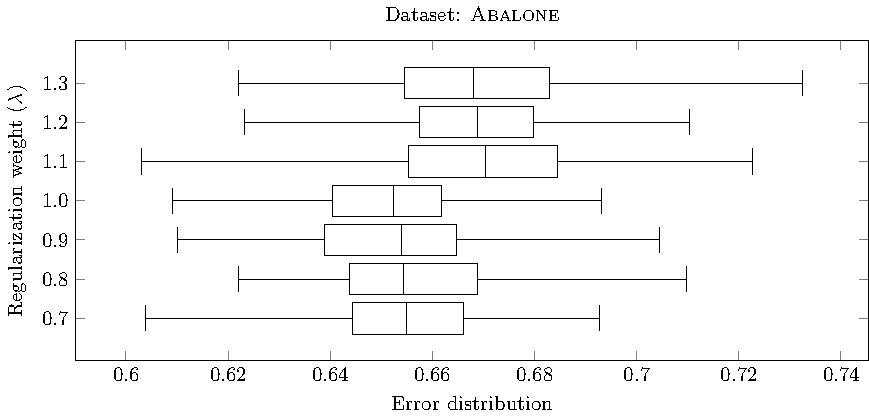
\includegraphics[width=0.48\textwidth]{Fig1a.pdf}
&
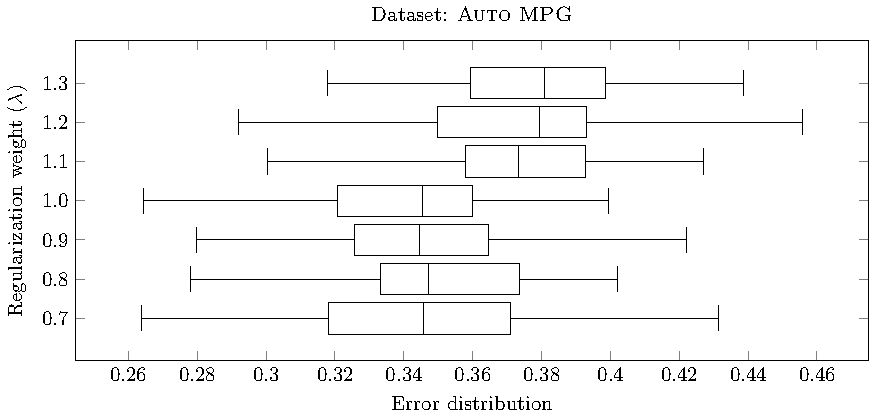
\includegraphics[width=0.48\textwidth]{Fig1b.pdf}
\\
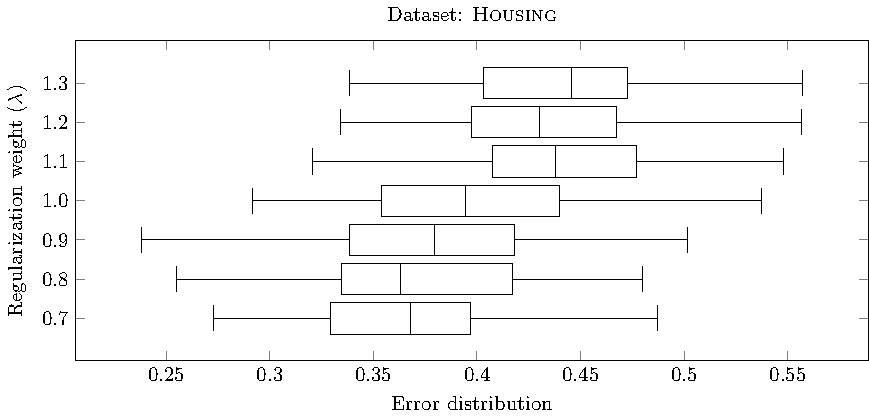
\includegraphics[width=0.48\textwidth]{Fig1c.pdf}
&
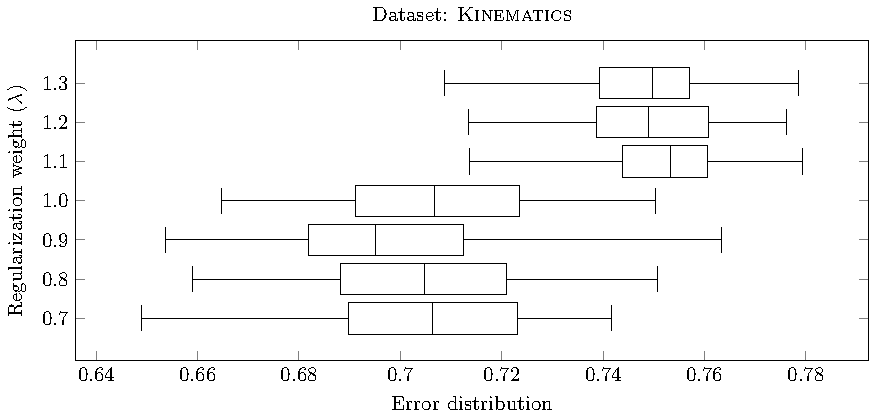
\includegraphics[width=0.48\textwidth]{Fig1d.pdf}
\end{tabular}

\caption{Error distribution by regularization exponent for common datasets. The box plots summarize error values of 75 simulations (60 iterations on a population size of 50) for each value of $\lambda$. Performance of the non-regularized \ac{EPR} is plotted in the line $\lambda = 1$. Performance for $\lambda < 1$ is better than $\lambda > 1$ in all datasets.}
\label{fig:lambda.error-distribution}\label{Abalone_dataset_lambdas}\label{Auto-MPG_dataset_lambdas}

\end{center}\end{figure*}

A simple exploration on the effect of the regularization parameter is depicted in Figure~\ref{fig:lambda.error-distribution} where it is possible to observe that penalizing polynomial complexity (i.e. $\lambda < 1$) achieves better results than the opposite ($\lambda > 1$). This observation motivates further inquire, done in section~\ref{sec:experimental.results}.\revised{please clarify this paragraph and justify this claim}{we rephrased the statement.}

\subsection{Genetic Algorithm Parameterization}

\revised{Please indicate all these values in detail}{We described the parameterization in more detail.}

\revised{You should contrast obtained results in a table.  Results are hard to judge from Fig 3 alone.}{Done that.}

\revised{The number of 250 for iterations seems premature specially when one looks at Fig 4. Stabilize? Really?  This only seems valid in one case of lambda.}{we changed the number of iterations to 2000, way behind stabilization}

In general \acp{GA} offer many possibilities with respect to the choice of genetic operators and respective application rates, population evolution, \emph{etc}. The results found here where obtained using the package \texttt{genalg}~\citep{Willighagen:2012aa} with standard operators (crossover and mutation) and population evolution defined by mutation rate of 5\% and 20\% elitism between generations.

\section{Experimental Results}\label{sec:experimental.results}

\begin{table}[t]
	\footnotesize
	\renewcommand{\arraystretch}{0.5}
	\begin{tabular}{ll|ccc}
		&&& \textbf{error} \\
		\textbf{dataset} & \textbf{method} & \textbf{quantile 25\%} & \textbf{mean} & \textbf{quantile 75\%} \\
		\hline
		Abalone	 & EPRR $\lambda = 0.7$ 	& 0.6392 & 0.6555 & 0.6677 \\
					 & EPRR $\lambda = 0.8$ 	& 0.6408 & 0.6543 & 0.6636 \\
					 & EPRR $\lambda = 0.9$ 	& 0.6481 & 0.6581 & 0.6707 \\
					 & EPRR $\lambda = 1.0$ 	& 0.6542 & 0.6715 & 0.6816 \\
					 & Linear Regression 	& 0.6803 & 0.6927 & 0.7078 \\
					 & SVM (linear kernel) 	& 0.6916 & 0.7044 & 0.7205 \\
					 & Regression Trees 	& 0.7423 & 0.7520 & 0.7621 \\
					 & Random Forest 	& 0.6585 & 0.6695 & 0.6814 \\
					 & Cond. Inference Trees 	& 0.7031 & 0.7126 & 0.7264 \\
		Auto-Mpg	 & EPRR $\lambda = 0.7$ 	& 0.3635 & 0.3916 & 0.4147 \\
					 & EPRR $\lambda = 0.8$ 	& 0.3629 & 0.3956 & 0.4228 \\
					 & EPRR $\lambda = 0.9$ 	& 0.3646 & 0.4130 & 0.4215 \\
					 & EPRR $\lambda = 1.0$ 	& 0.3691 & 0.3999 & 0.4057 \\
					 & Linear Regression 	& 0.4071 & 0.4284 & 0.4473 \\
					 & SVM (linear kernel) 	& 0.4116 & 0.4358 & 0.4613 \\
					 & Regression Trees 	& 0.4216 & 0.4501 & 0.4785 \\
					 & Random Forest 	& 0.3318 & 0.3624 & 0.3892 \\
					 & Cond. Inference Trees 	& 0.4063 & 0.4372 & 0.4663 \\
		Housing	 & EPRR $\lambda = 0.7$ 	& 0.4412 & 0.6650 & 0.5739 \\
					 & EPRR $\lambda = 0.8$ 	& 0.4241 & 0.5274 & 0.6016 \\
					 & EPRR $\lambda = 0.9$ 	& 0.4354 & 0.5717 & 0.6462 \\
					 & EPRR $\lambda = 1.0$ 	& 0.4477 & 0.5417 & 0.5995 \\
					 & Linear Regression 	& 0.4898 & 0.5313 & 0.5649 \\
					 & SVM (linear kernel) 	& 0.4831 & 0.5469 & 0.6017 \\
					 & Regression Trees 	& 0.4845 & 0.5232 & 0.5720 \\
					 & Random Forest 	& 0.3283 & 0.3679 & 0.4023 \\
					 & Cond. Inference Trees 	& 0.4676 & 0.5080 & 0.5413 \\
		Kinematics	 & EPRR $\lambda = 0.7$ 	& 0.6600 & 0.6660 & 0.6720 \\
					 & EPRR $\lambda = 0.8$ 	& 0.6617 & 0.6694 & 0.6751 \\
					 & EPRR $\lambda = 0.9$ 	& 0.6636 & 0.6714 & 0.6761 \\
					 & EPRR $\lambda = 1.0$ 	& 0.7568 & 0.7558 & 0.7739 \\
					 & Linear Regression 	& 0.7672 & 0.7759 & 0.7849 \\
					 & SVM (linear kernel) 	& 0.8074 & 0.8136 & 0.8247 \\
					 & Regression Trees 	& 0.5673 & 0.6021 & 0.5803 \\
					 & Random Forest 	& 0.7386 & 0.7344 & 0.7645 \\
					 & Cond. Inference Trees 	& 0.7558 & 0.7620 & 0.7686
	\end{tabular}
	\caption{Tabular summary results for different regression methods on common datasets. Although \ac{EPRR} not always achieves the smallest expected error, performance is on-par with more sophisticated methods.}
\end{table}
Here is described the experiment setup used to gather and summarize the empirical evidence that supports this comparative study of \ac{EPR} and \ac{EPRR}. Evaluation is focused in \ac{rmse} distribution and, besides \ac{EPR} and \ac{EPRR}, also uses several common regression methods and datasets easily accessible in \texttt{R}, the free software environment for statistical computing and graphics~\citep{R-Core-Team:2013aa}\footnote{The datasets and \texttt{R} code used to produce the results and plots in this paper are available online at \url{https://github.com/jpneto/GenAlgPoly}.}. A small consideration on the convergence speed concludes this section.

\subsection{Regression Methods and Datasets}

The \ac{EPRR} method is ranked against several well-known learning algorithms for regression, namely: non-regularized \ac{EPR}, Linear Regression, Support Vector Machines~\citep{Meyer:2012aa} with linear kernel, Regression Trees~\citep{Therneau:2013aa}, Random Forest~\citep{Strobl:2008aa,Strobl:2007aa} and Conditional Inference Trees~\citep{Hothorn:2006aa}.
%
%	INCLUDE ?
%
%To achieve better error results the \ac{SVM} and Regression Tree parameters are tuned in each dataset.

The performance of each method is evaluated on several common datasets. From each dataset 70\% of the observations are reserved for training purposes and the remaining observations used to estimate the \ac{rmse}. To enhance the robustness of results this process is repeated $25$~times, each time with a different shuffling of the samples in the train and test sets. Some datasets with attribute values of different magnitudes have a pre-processing scaling transformation. The box plots in figures \ref{artificial_dataset1_lambda1.0} and \ref{fig:four.datasets.summary} resume the test set error distributions over these different runs.

One of the used datasets, \textsc{Artificial}, has a special role: it is used to test if \ac{EPRR} is able to discover a polynomial model. The idea of this test is to generate a polynomial dependent variable and measure the \ac{EPRR} \ac{rmse} after fitting the dataset. The genetic algorithm parameterization for this dataset uses a population with size $n=100$ and evolves for $50$~generations. For the remaining datasets the population has size~$n=300$ and evolves for $100$~generations.

\begin{figure*}[tb]\begin{center}
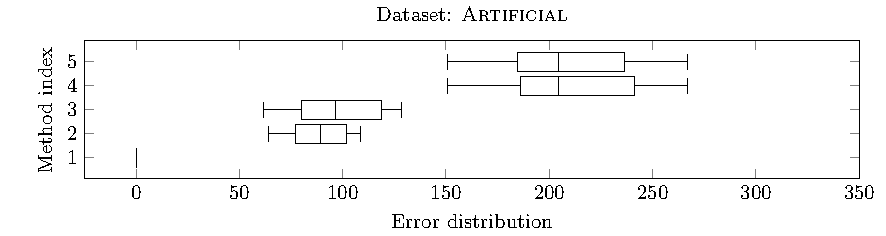
\includegraphics[width=0.98\textwidth]{figure_2.pdf}
\caption{Testing polynomial discovery. The dataset is generated from a polynomial expression and, as shown, \ac{EPRR} finds the exact generator structure: in line 1, the error box is centered in $0$ and has width $0$.  The regression methods depicted are: 1. \ac{EPRR}, 2. Linear Regression, 3. SVM, 4. Regression Trees and 5. Conditional Inference Trees}
\label{artificial_dataset1_lambda1.0}
\end{center}
\end{figure*}

\begin{description}
\item{\textsc{Artificial}} is a polynomial dataset with four numeric features, $x_1, \ldots x_4$, where $x_1,x_3$ are outcomes from Poisson random variables, and $x_2,x_4$ from Normal random variables. The dependent variable is given by the polynomial expression $y = x_2x_4^2 + x_1^2x_3 + 5$. The dataset includes $n=50$~observations;

\item{\textsc{Housing}} concerns the task of predicting housing values in areas of Boston. There are $n=506$ observations of $m=13$ continuous attributes and one dependent variable, the median value of owner-occupied homes in thousands of USD;


\item{\textsc{Abalone}} is used to predict the age of a abalone shell using $m=8$ numeric attributes concerning several physical measurements. There are $n=4177$ observations;

\item{\textsc{Auto MPG}} gathers fuel consumption in miles per gallon, based on two discrete and five continuous attributes ($m=7$). There are $n=398$ observations;

\item{\textsc{Kinematics}} results from a realistic simulation of the forward kinematics of an 8 link robot arm. The task is to predict the distance of the end-effector from a target using $m=8$ continuous attributes. There are $n=8192$ observations;

\end{description}
%
\begin{figure*}[tb]\begin{center}
\begin{tabular}{cc}
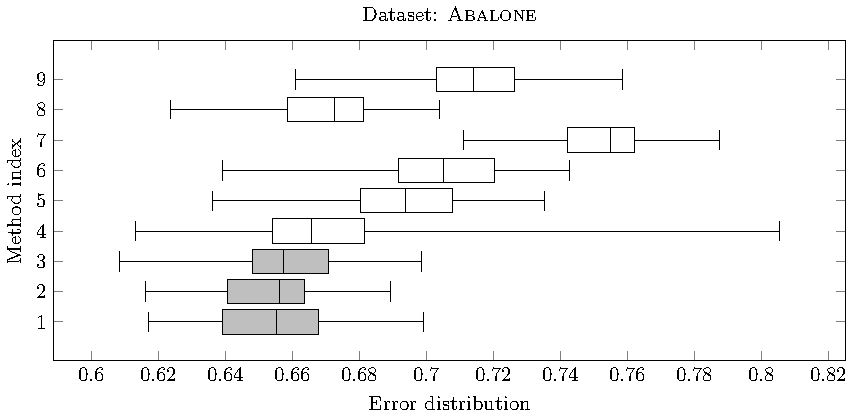
\includegraphics[width=0.48\textwidth]{Fig3a.pdf}
&
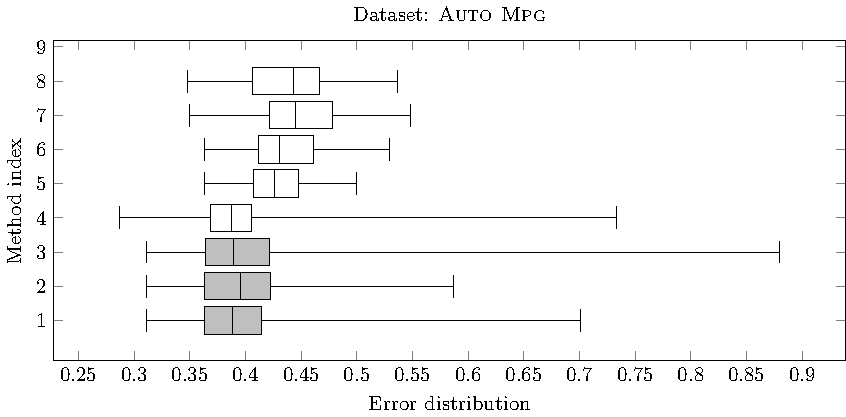
\includegraphics[width=0.48\textwidth]{Fig3b.pdf}
\\
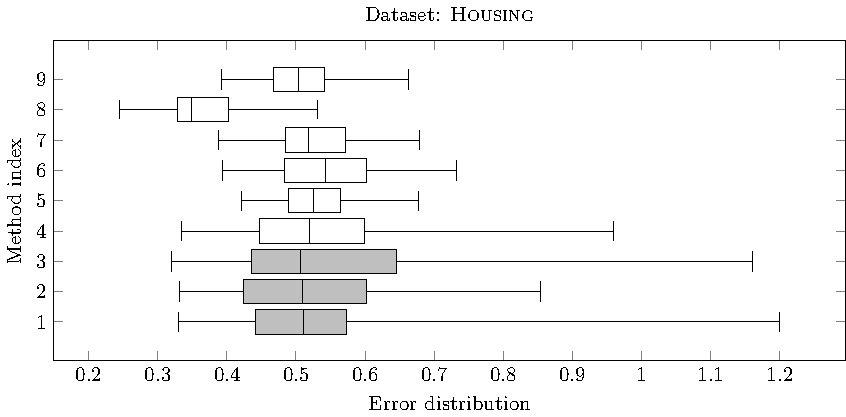
\includegraphics[width=0.48\textwidth]{Fig3c.pdf}
&
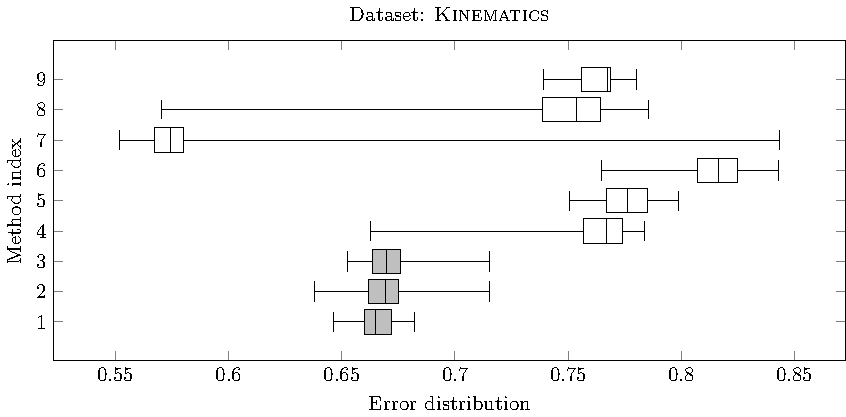
\includegraphics[width=0.48\textwidth]{Fig3d.pdf}
\end{tabular}
%
\caption{Graphical summary results for different regression methods on common datasets. Although \ac{EPRR} not always achieves the smallest expected error, performance is on-par with more sophisticated methods.  The regression methods depicted in these figures are:
1. \ac{EPRR}, $\lambda = 0.7$;
2. \ac{EPRR}, $\lambda = 0.8$;
3. \ac{EPRR}, $\lambda = 0.9$;
4. \ac{EPR} (i.e. $\lambda = 1.0$);
5. Linear Regression;
6. \ac{SVM} (linear kernel);
7. Regression Trees;
8. Random Forest (with 100 trees);
9. Conditional Inference Trees.}
\label{fig:four.datasets.summary}
\label{Housing_dataset_lambda0.8_25runs}
\label{Abalone_dataset_lambda0.8_25runs}
\label{Auto-Mpg_dataset_lambda0.8_25runs}
\label{Kinematics300_lambda0.8_25runs}
\end{center}\end{figure*}

\subsection{Convergence speed}
%
\begin{figure*}[tb]
	\begin{center}
		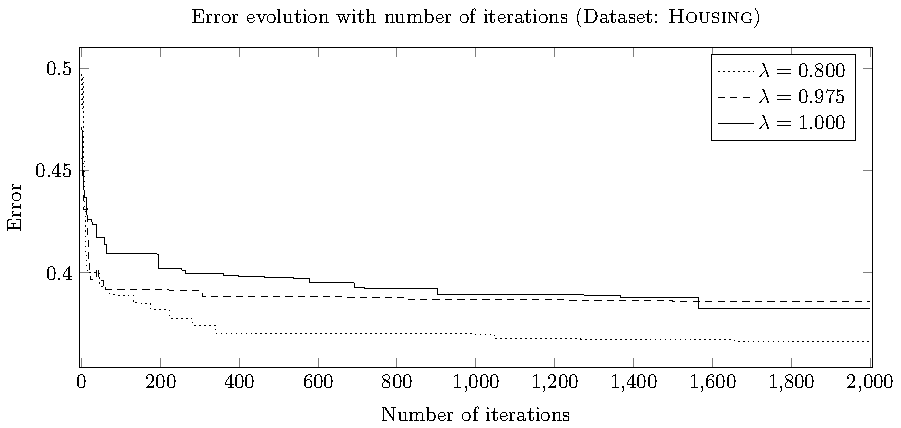
\includegraphics[width=0.98\textwidth]{Fig4xx.pdf}
		\caption{Learning curve: Error progress for the \textsc{Housing} dataset during a single execution of the genetic algorithm. The figure shows the fitness evolution for different regularization values. The population of each run consists of $200$ polynomials.}
		\label{Abalone_fitnessProgress}
	\end{center}
\end{figure*}
%
Since this work is oriented to the \ac{rmse} of the \ac{EPRR} model it is necessary to assess how this depends on the number of generations of the \ac{GA}. As illustrated in Figure~\ref{Abalone_fitnessProgress}, the \ac{rmse} quickly drops during the initial $50$ to $100$ generations. Then, it proceeds slower achieving better solutions only with marginal error reduction.

\section{Conclusion and Future Work}

Of the regression methods considered \ac{SVM} achieves the best results in three out of four datasets. However \ac{SVM} and Conditional Inference Trees are pre-trained, having parameters tuned for each particular dataset unlike \ac{EPRR}, that runs with the same parameterization on all datasets. Even so it is the best estimator for the \textsc{Abalone} dataset and in the remaining datasets it outperforms most of the other estimators. 

Comparing \ac{EPR} and \ac{EPRR} --- the main article's topic --- the regularized version achieves much better results at \textsc{Abalone} and especially \textsc{Kinematics}. On the \textsc{Housing} dataset errors are improved  wrt \ac{EPR} in a difference in means, resulted in a 95\% HDI (Highest Density Interval) equal to $\left\lbrack 0.001, 0.119 \right\rbrack$ which, while borderline, achieves statistical significance. Only in the \textsc{Auto MPG} dataset \ac{EPR} achieves better results, even if not that different from \ac{EPRR}.

For complexity considerations \ac{EPR} and \ac{EPRR} demand some processing time. On a quad-core computer, processing the \textsc{Kinematics} dataset (with near $8K$~observations) takes approximately 5~minutes. Probably processing time can be reduced by one to two orders in magnitude if the algorithm is implemented with computational speed in mind. However, speed optimization is not the focus of this article.

A cross-validation procedure can be implemented to refine the appropriate parameter values to achieve better errors. Namely, the regularization parameter, $\lambda$, can be tested with several values, instead of being fixed at $0.8$. Other parameters like mutation chance or the amount of elitism can also be tested. However, these type of tests need a low-level, fast implementation of \ac{EPR} and are postponed to future investigation.

\section*{Acknowledgements}

The authors are grateful to the Fundação para a Ciência e Tecnologia (FCT) and the  R\&D laboratory LabMAg for the financial support given to this work, under the strategic project \textsc{PEst-OE/EEI/UI0434/2011}.

Datasets used herein are selected from Luís Torgo's data repository, \url{http://www.dcc.fc.up.pt/~ltorgo/Regression/DataSets.html}. Most can also be found in the UCI ML repository at \url{http://archive.ics.uci.edu/ml/}.

The authors wish to thank professor André Falcão for motivation and useful discussions around the article.

\bibliographystyle{plain}
\bibliography{fullbib2}
    
\end{document}